\section{Mise en contexte}
    Dans un contexte de robotique, la puissance de calcul et la mémoire sont limitées, il faut donc optimiser l'utilisation des ressources au maximum. Malheureusement, il est nécessaire d’avoir une vaste quantité de stimuli provenant de différents capteurs (caméra RGB, caméra 3D, LIDAR, matrice de microphones, ...) pour rendre un robot le plus autonome possible. Ainsi, il y a trop de stimuli pour faire un traitement détaillé de chacun de ceux-ci avec les ressources embarquées. Puisqu’il est fort probable que seulement un sous-ensemble des stimuli soit important à un moment donné, il n’est donc pas nécessaire de tous les traiter simultanément. Il est intéressant de jeter un coup d'oeil à l'humain pour savoir comment il arrive à gérer tous les stimuli. L’être humain possède un mécanisme d’attention sélective permettant de se concentrer sur les stimuli les plus utiles au moment présent.
    \bigskip
    
    L’architecture robotique HBBA (\textit{Hybrid Behavior-Based Architecture})  [1, 2, 3] possède un mécanisme d’attention sélective fonctionnant à l’aide de filtres à décimation. Par exemple, un filtre à décimation sur un signal vidéo permet de traiter une image sur \(N\), où \(N\) est un paramètre du filtre. Ce mécanisme d’attention sélective permet de réduire les ressources utilisées sur un robot pour permettre l’exécution d’autres traitements qu’il serait impossible de réaliser sans ce mécanisme. Dans l’architecture robotique HBBA, les filtres à décimation sont paramétrés par le développeur à l'aide de désirs et de stratégies. Il serait intéressant que le robot fasse cette paramétrisation de façon autonome. Un signal de curiosité serait en mesure de faire cela. Plus un stimulus possède un signal de curiosité élevé, plus le paramètre \(N\) de ce filtre doit être faible. Il est possible de  générer un signal de curiosité à l’aide d’un auto-encodeur. L’erreur de reconstruction d’un auto-encodeur peut être utilisée comme signal de curiosité. Si l'erreur de reconstruction est élevée pour un stimulus, alors le robot n'a jamais rencontré cette situation pour le sens (le capteur) d’où provient ce stimulus, donc le robot devrait être curieux pour ce sens. Pour que le robot soit en mesure ne pas donner son attention toujours au même stimulus, le signal de curiosité doit diminuer à force que le même stimulus est senti.
    \bigskip
    
    Pour utiliser un signal de curiosité pour la paramétrisation des filtres à décimation, il est important que la génération des signaux de curiosité n’utilise que peu de ressources. Il est possible d’utiliser des auto-encodeurs utilisant les données brutes des capteurs, mais ceci a le potentiel d’utiliser trop de ressources. La question suivante se pose : est-il possible d’utiliser des caractéristiques décrivant les stimuli au lieu des données brutes? La réponse est oui. Un réseau de neurones pourrait extraire des caractéristiques que l’auto-encodeur pourrait utiliser pour générer le signal de curiosité. Cette architecture de réseaux de neurones a été utilisée dans un contexte d’exploration d’un environnement à l’aide d’apprentissage par renforcement et d’un signal de curiosité [4]. L’utilisation de caractéristiques au lieu des pixels leur a permis d’améliorer les performances. Pour assurer la diminution du signal de curiosité dans le temps, l’entraînement des réseaux de neurones doit se faire en ligne. L’apprentissage se fait de manière non supervisée en diminuant les signaux de curiosité (erreurs de reconstruction).

\section{Définition du projet}
    \label{sec:definition_projet}
    Afin de respecter le temps qu’il est possible d’accorder au projet, le générateur de signaux de curiosité sera implémenté pour un cas d’utilisation simplifié. Les stimuli seront des images RGB provenant d’une caméra filmant en  Full HD (1920x1080). Les images Full HD seront divisées en 144 régions de 120x120 pixels qui seront considérés comme des images provenant de caméras différentes. Les images de ces régions seront des stimuli à part entière. Pour simplifier le projet, une région peut avoir l’attention ou non (\(N = \infty\)). Aucune attention partielle ne sera considérée. L’objectif est donc d’indiquer au robot une zone approximative de l’image Full HD où il doit focaliser son attention. Dans le cas non simplifié, l’objectif serait de changer le paramètre \(N\) de chacun des filtres à décimation de chaque stimulus en fonction de la valeur du signal de curiosité pour ce stimulus (chaque capteur génère un seul stimulus).
    
    Par exemple, si notre modèle est entraîné sur des images de murs sans affiche, alors une affiche sur un mur générerait des signaux de curiosité élevés pour les régions contenant l’affiche. L’attention sera donnée aux régions ayant un signal de curiosité supérieur à un certain seuil. Par conséquent, les régions correspondantes à l’affiche devraient avoir l’attention afin que le robot puisse traiter ces stimuli (par exemple, pour s’orienter vers l’affiche ou pour analyser le texte sur l’affiche). La figure \ref{fig:definition_sortie_reseau} présente l’exemple énoncé. 
    
    \pagebreak
    \begin{figure}[H]
        \centering
        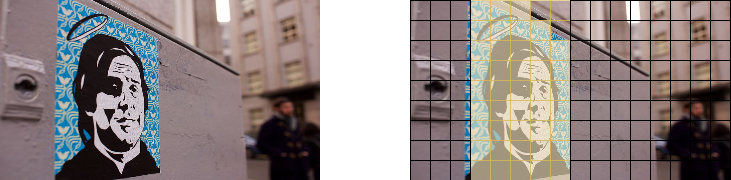
\includegraphics[width=15cm]{images/definition.png}
        \caption[Définition de la sortie du réseau]{Définition de la sortie du réseau\footnotemark}
        \label{fig:definition_sortie_reseau}
    \end{figure}
    \footnotetext{\url{https://www.peakpx.com/431428/pop-art-painting-on-white-wall}}